\xpartbox{Application/Software}

\begin{xpsectionbox}{}{}

\begin{minipage}{0.4\linewidth}
\begin{itemize}
	\item important/helpful in disaster scenarios
	\item complementarity between text and images
	\item web interface
		\begin{itemize}
			\item intuitive
			\item accessibility from remote places
		\end{itemize}
\end{itemize}
\end{minipage}
\begin{minipage}{0.6\linewidth}
\begin{center}
	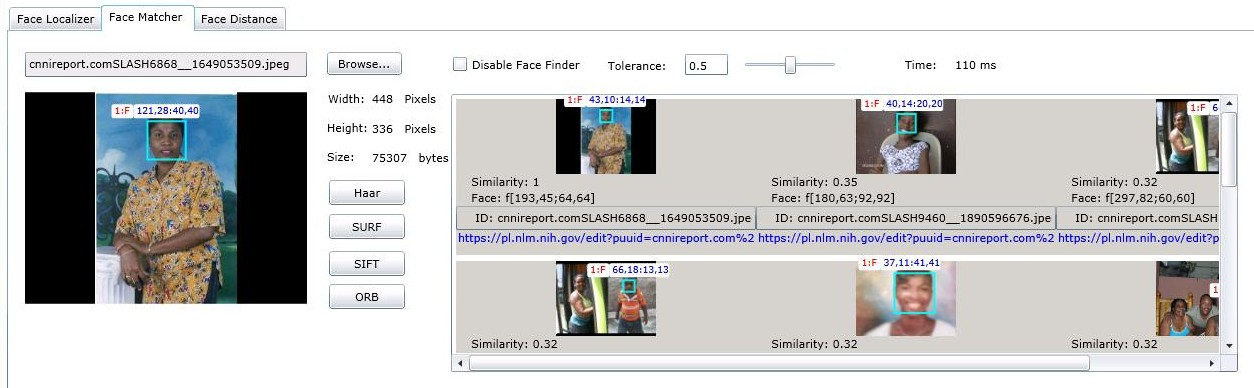
\includegraphics[height=0.5\linewidth]{images/web_interface}
\end{center}
\end{minipage}

%\begin{minipage}{0.4\linewidth}
%
%\begin{itemize}
%	  \item low-level image features (Haar, LBP, etc.)
%	  \item high-level facial landmarks (eye(s), nose, mouth, ear(s), chin, etc.)
%	  \item skin color
%\end{itemize}
%\end{minipage}
%\begin{minipage}{0.6\linewidth}
%
%\begin{center}
%%			%\hspace{-5cm}
%%			\vspace{-1cm}
%			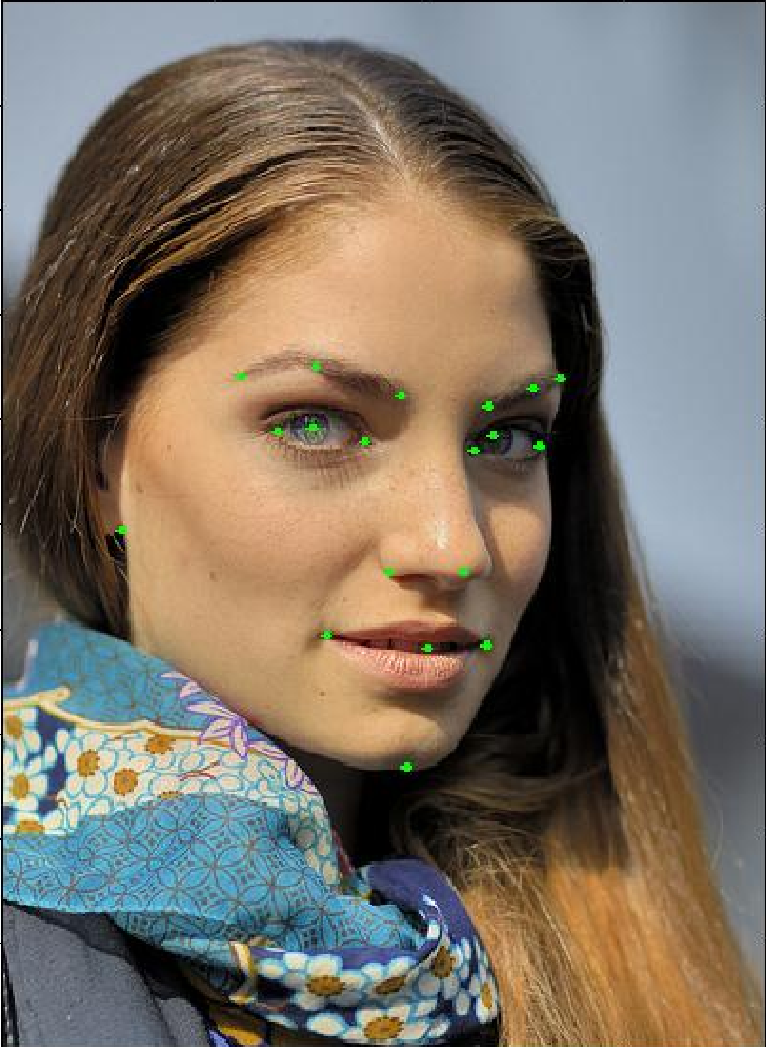
\includegraphics[height=0.25\linewidth]{images/facial_landmarks}
%			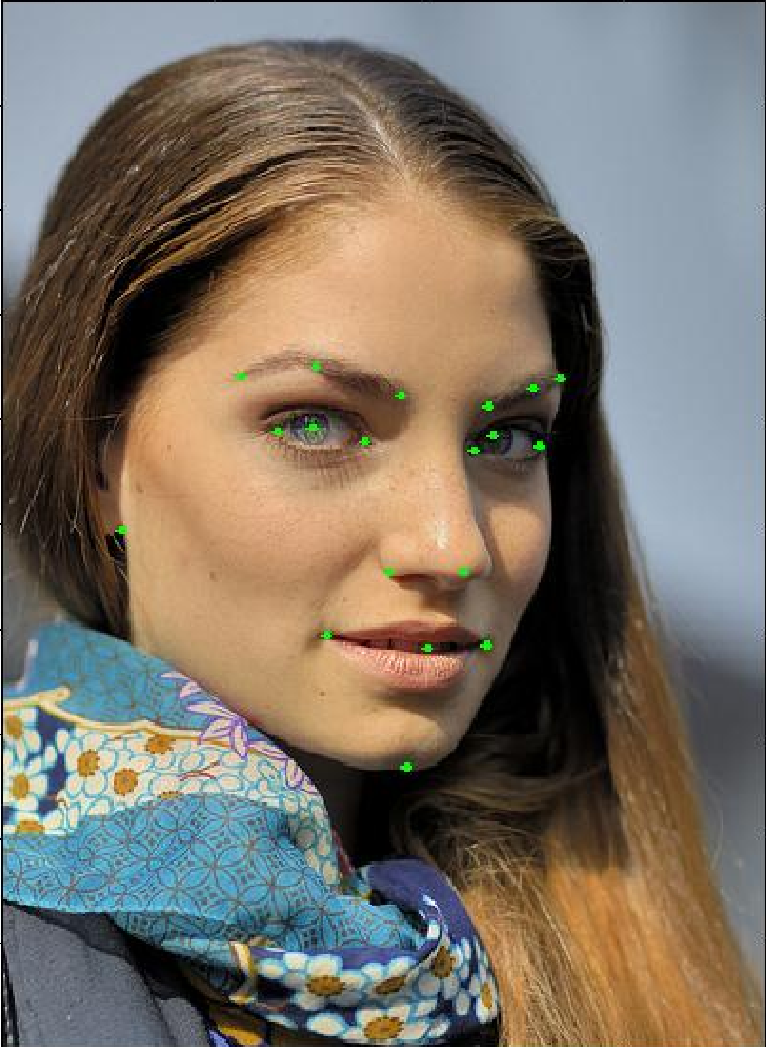
\includegraphics[height=0.25\linewidth]{images/facial_landmarks}
%\end{center}
%
%\end{minipage}
%\end{xpsectionbox}
%
%\begin{xpsectionbox}{Challenges}{}
%
%\begin{minipage}{0.4\linewidth}
%\begin{itemize}
%	  \item low-quality images
%	  \item various lighting conditions
%	  \item frontal vs. profile faces
%	  \item various skin colors
%	  \item occlusions, facial hair, spectacles, hat, etc.
%\end{itemize}
%\end{minipage}
%\begin{minipage}{0.6\linewidth}
%\begin{center}
%			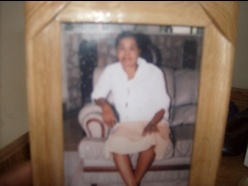
\includegraphics[height=0.25\linewidth]{images/PL_low_quality}
%			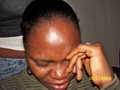
\includegraphics[height=0.25\linewidth]{images/HEPL_occlusion}
%			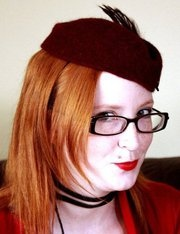
\includegraphics[height=0.25\linewidth]{images/HEPL_spectacles_hat}
%\end{center}
%\end{minipage}

\end{xpsectionbox}